\section{Outreach} \label{sec:appE}

\subsection{Outreach on Project Website}

To increase the projects out reach the TUBULAR Team created a project website. On the website there are descriptions of the project, a link to download the latest SED, information on the TUBULAR Team members and sponsors and a contact link. In addition the microblogging carried out by the TUBULAR Team is also displayed on the website.

\begin{figure}[H]
    \centering
    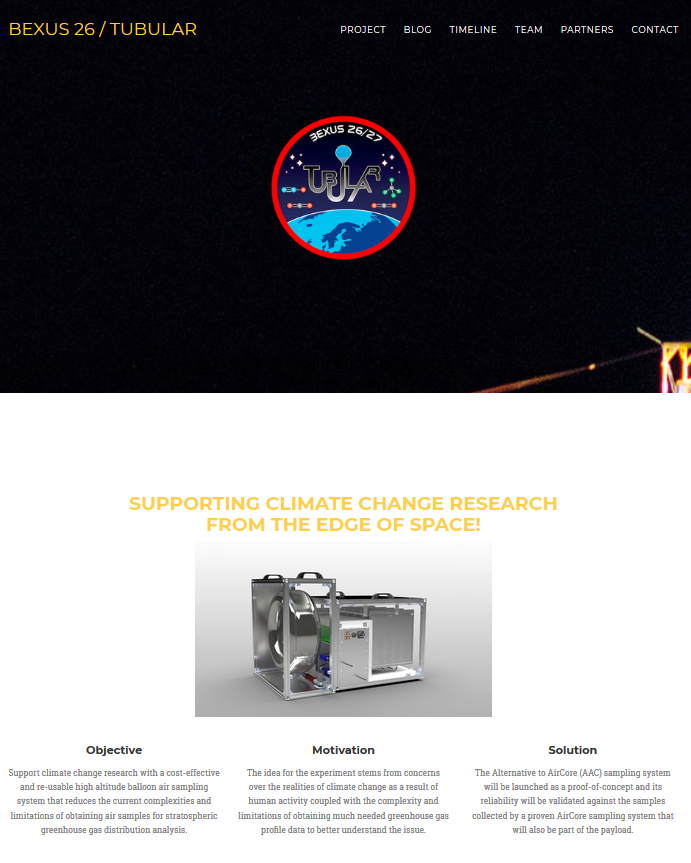
\includegraphics[width=0.9\linewidth]{appendix/img/outreach/outreach-tubwebsite-front.PNG}
    \caption{The Home Page of TUBULAR's Website.}
    \label{fig:outreach-tubwebsite}
\end{figure}
\begin{figure}[H]
    \begin{align*}
        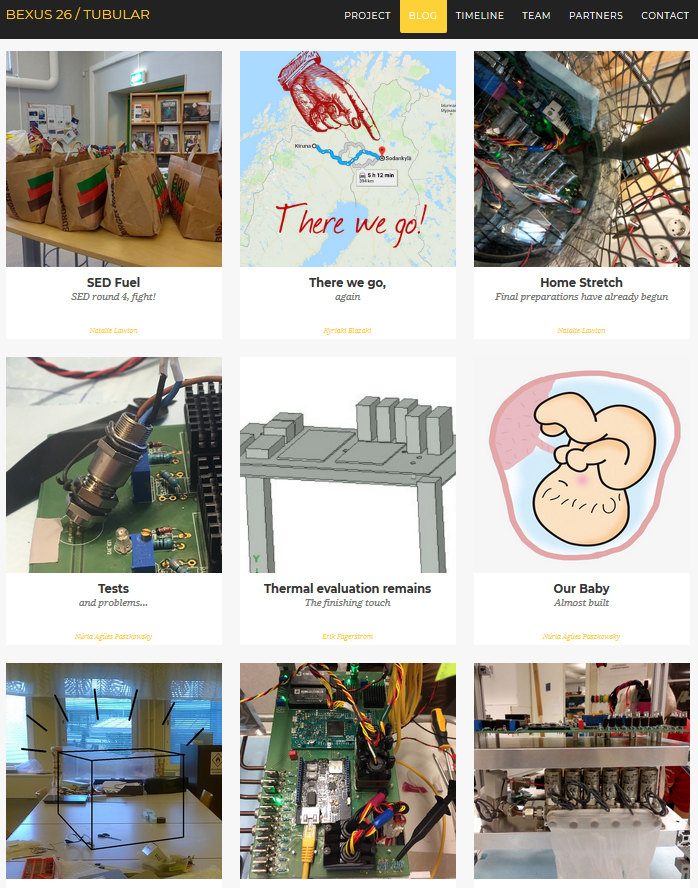
\includegraphics[width=1\linewidth]{appendix/img/outreach/outreach-tubwebsite-inside.PNG}
    \end{align*}
    \caption{The Daily Microblogging Displayed on the Website.}
    \label{fig:outreach-microblog}
\end{figure}
\begin{figure}[H]
    \begin{align*}
        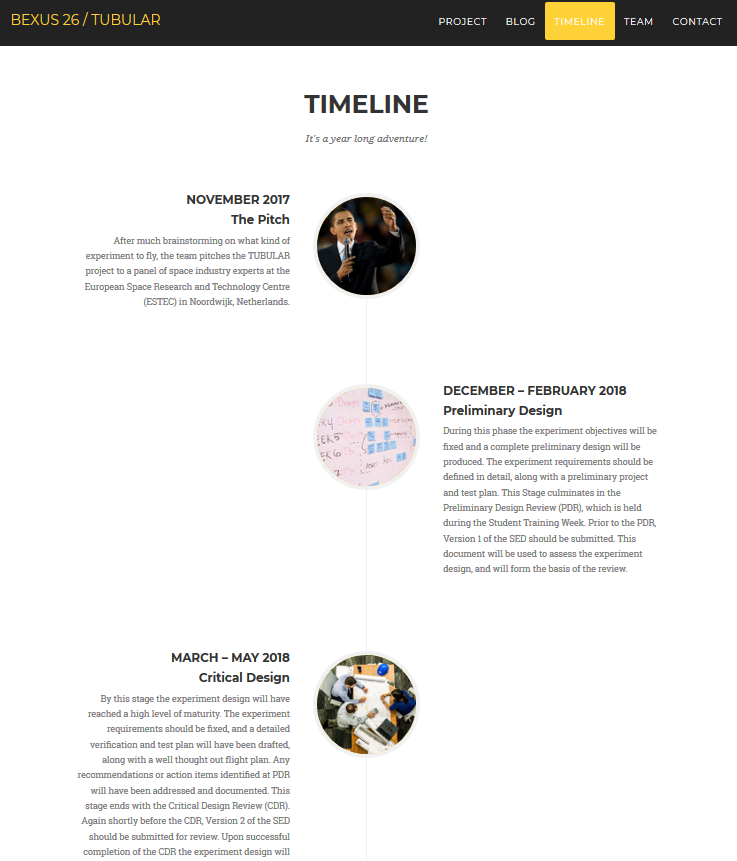
\includegraphics[width=1\linewidth]{appendix/img/outreach/outreach-tubwebsite-timeline.PNG}
    \end{align*}
    \caption{The Timeline for This Project Available on the Website.}
    \label{fig:outreach-timeline}
\end{figure}
\begin{figure}[H]
    \begin{align*}
        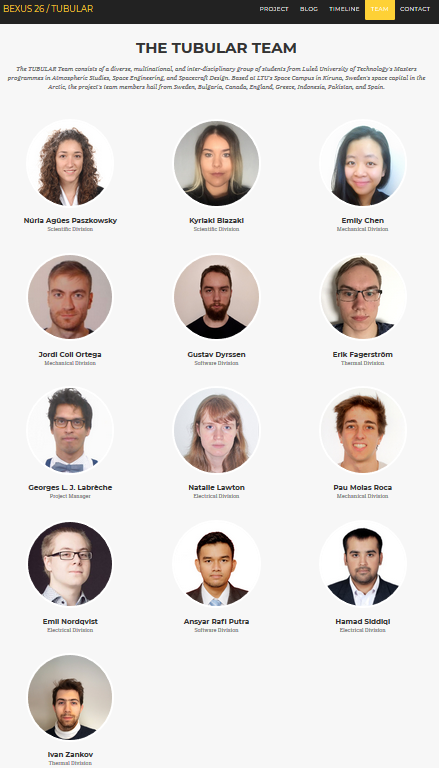
\includegraphics[width=0.8\linewidth]{appendix/img/outreach/outreach-tubwebsite-team.PNG}
    \end{align*}
    \caption{The Information of the Tubular's Team Members Available on the Website.}
    \label{fig:outreach-team}
\end{figure}
\begin{figure}[H]
    \begin{align*}
        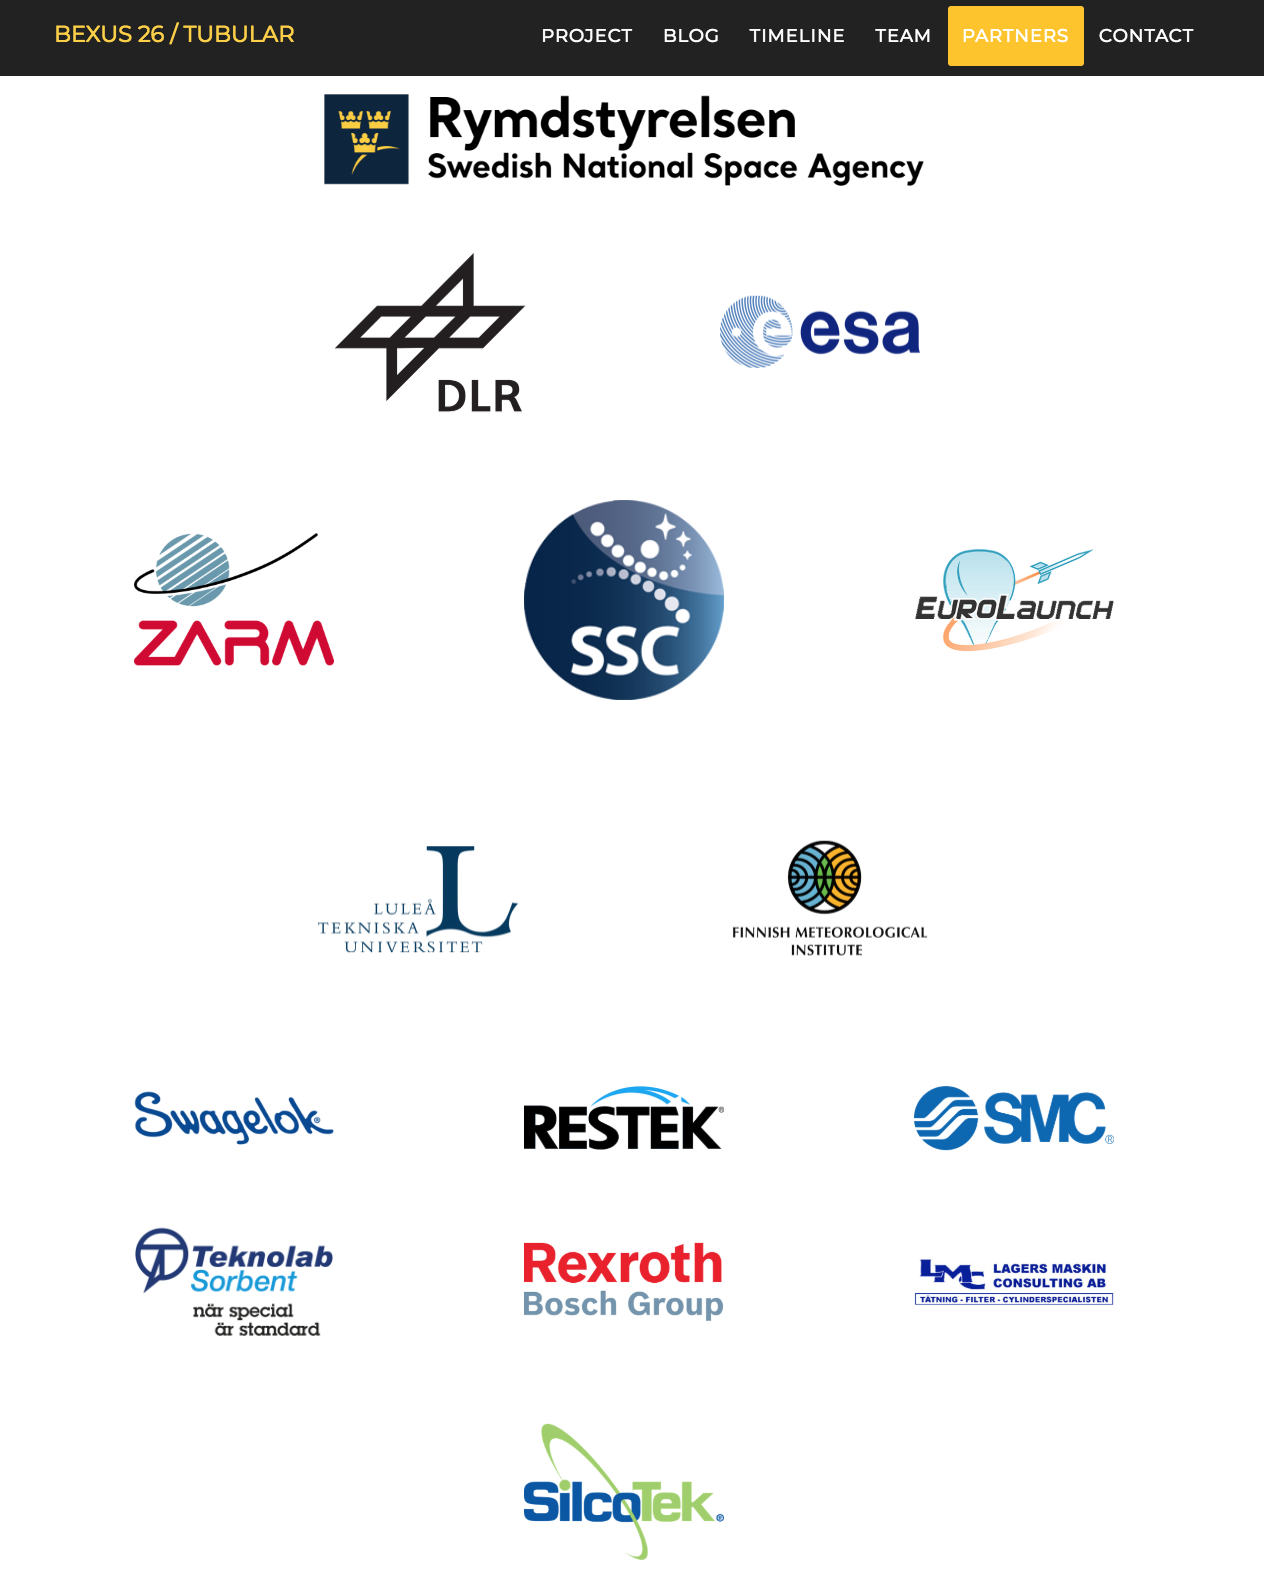
\includegraphics[width=1\linewidth]{appendix/img/outreach/outreach-tubwebsite-spons.PNG}
    \end{align*}
    \caption{The Sponsors In This Project Available on the Website.}
    \label{fig:outreach-spons}
\end{figure}

\begin{landscape}
\subsection{Outreach Timeline}
\begin{figure}[H]
    \centering
    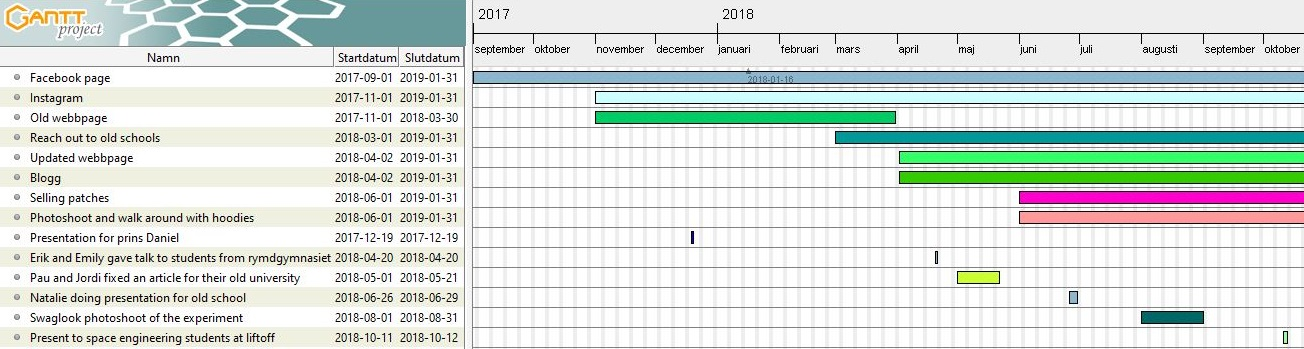
\includegraphics[width=1.5\textwidth]{appendix/img/outreach/outreach-timeline.jpg}
    \caption{Outreach Timeline for the Whole BEXUS Project.}
    \label{fig:outreach-timeline}
\end{figure}
\end{landscape}

\newpage
\subsection{Social Media Outreach on Facebook}

Another outreach avenue is Facebook. On Facebook the TUBULAR Team posts photos, short text updates and links to our blog posts. 

\begin{figure}[H]
    \begin{align*}
        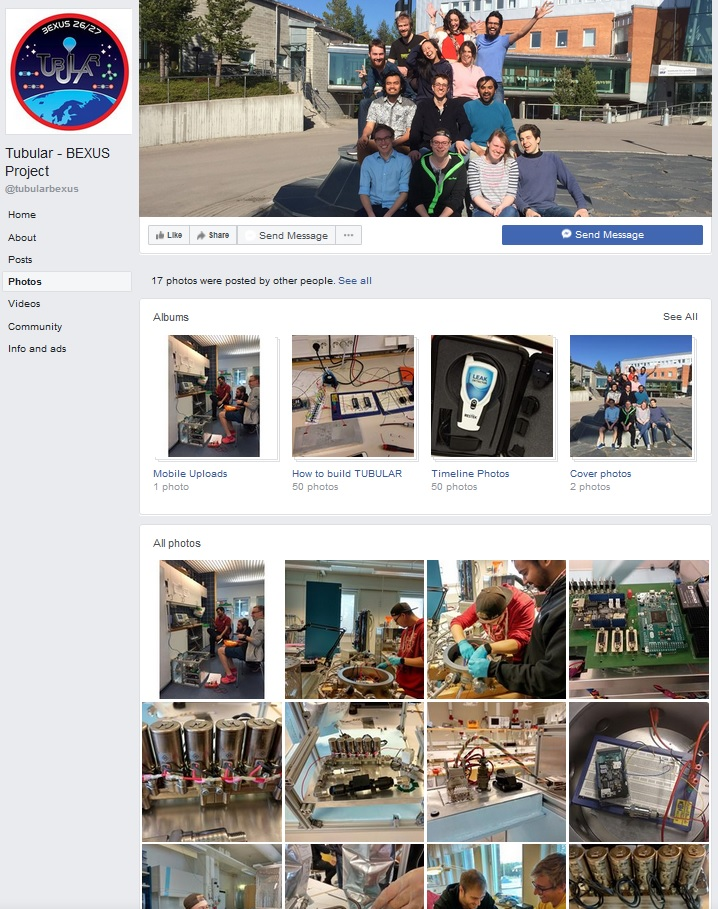
\includegraphics[width=0.8\linewidth]{appendix/img/outreach/outreach-facebook.jpg}
    \end{align*}
    \caption{Photos from Social Media Outreach on Facebook.}
    \label{fig:outreach-facebook}
\end{figure}

\newpage
\subsection{Social Media Outreach on Instagram}

On Instagram the TUBULAR Team posts regularly with updates on the project progress and what the TUBULAR Team has been up to.

\begin{figure}[H]
    \begin{align*}
        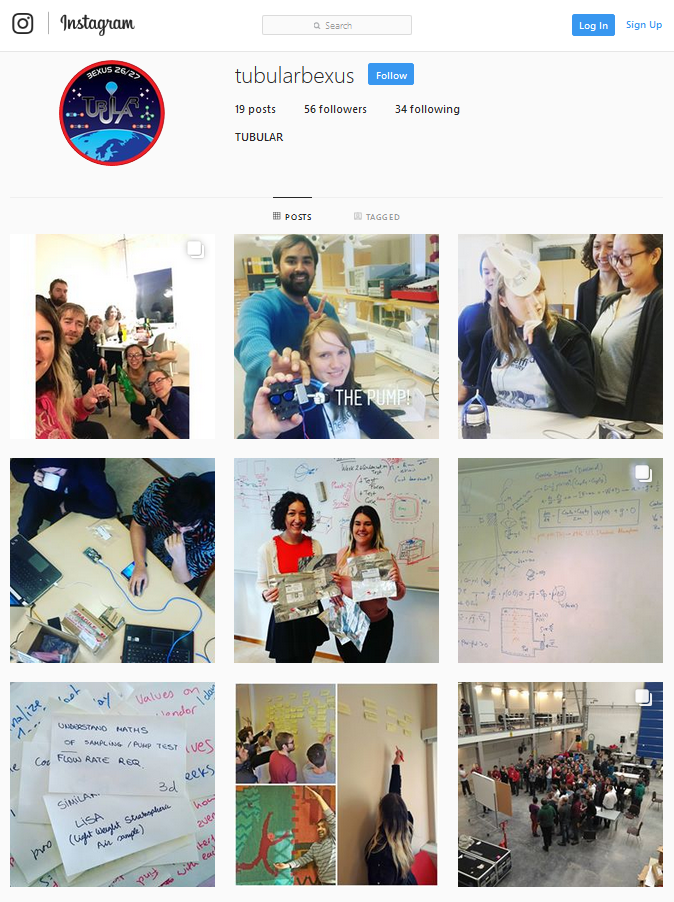
\includegraphics[width=0.9\linewidth]{appendix/img/outreach/outreach-instagram.PNG}
    \end{align*}
    \caption{Some of the Social Media Outreach on Instagram.}
    \label{fig:outreach-instagram}
\end{figure}

\newpage
\subsection{Outreach with Open Source Code Hosted on a REXUS/BEXUS GitHub Repository}

The TUBULAR Team has opened a GitHub Repository to share all the code used in the TUBULAR project. It was created with an open invite to all other REXUS/BEXUS teams to view, use and contribute to.
\begin{figure}[H]
    \begin{align*}
        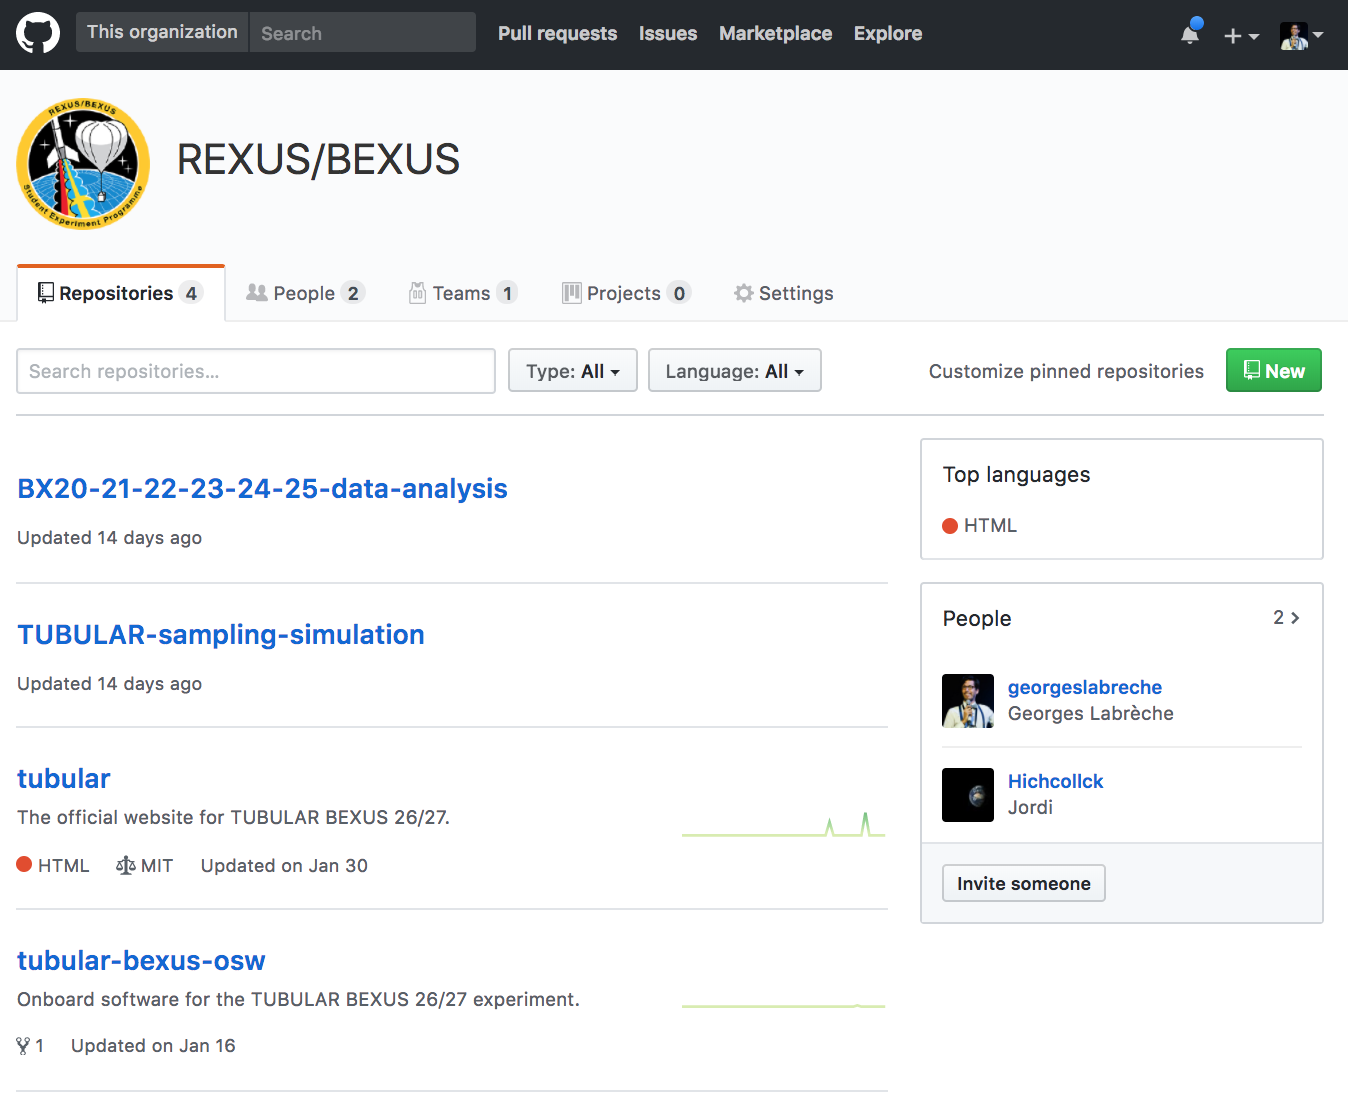
\includegraphics[width=0.6\linewidth]{appendix/img/outreach/outreach-github.png}
    \end{align*}
    \caption{The Open Source Code Hosted on a REXUS/BEXUS GitHub Repository.}
    \label{fig:outreach-github}
\end{figure}

\subsection{Outreach with Team Patch}

The team also had patches made of the TUBULAR logo and 150 patches have been ordered. Around 70 of these have already been bought by the team for themselves and to give to friends and family. It is intended that the remaining 80 will be sold for a small profit at university.

\begin{figure}[H]
    \begin{align*}
        
\includegraphics[width=0.3\textwidth]{appendix/img/outreach/outreach-patch.png}
    \end{align*}
    \caption{A Photo of the Patch in Production Sent by the Company Making it.}
    \label{fig:outreach-patch}
\end{figure}

\subsection{Visit by the Canadian Ambassador}
During Canadian Ambassador Heather Grant's visit at the Swedish Institute of Space Physics, the team got the honor to do a brief presentation of the TUBULAR project. It also included a short explanation regarding one of the electrical tests in the vacuum chamber. This is now displayed on the universities website with a link to the TUBULAR website.

\begin{figure}[H]
    \begin{align*}
        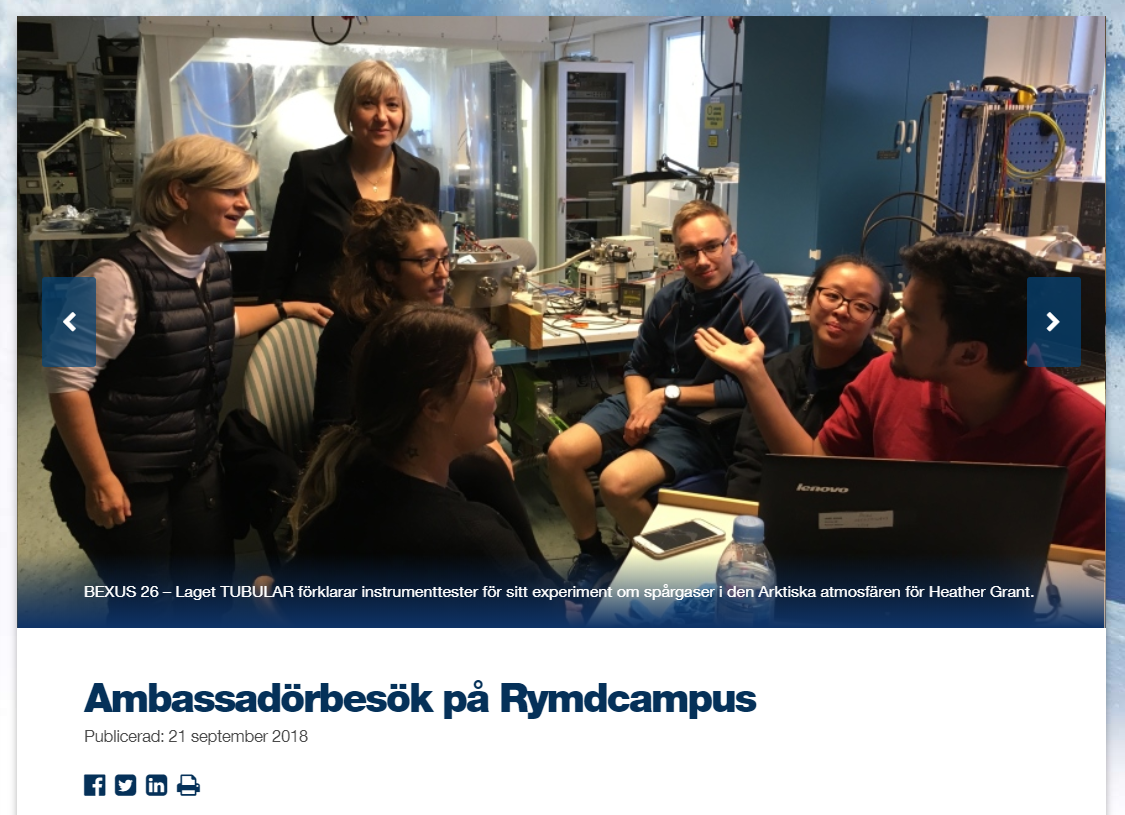
\includegraphics[width=0.8\textwidth]{appendix/img/outreach/ambassardor.png}
    \end{align*}
    \caption{Picture taken by Ella Carlsson which is shown on the LTU Website.}
    \label{fig:outreach-patch}
\end{figure}

\begin{figure}[H]
    \begin{align*}
        
\includegraphics[width=0.8\textwidth]{appendix/img/outreach/amabadasoiashdna.png}
    \end{align*}
    \caption{The Text Accomopanying the Image on the LTU Webpage.}
    \label{fig:outreach-patch}
\end{figure}


\subsection{Attendance at Lift Off 2018}
The team will attend Lift Off 2018 event and present the TUBULAR project for students, companies and organizations. The guests will have a chance to have a peek at the whole experiment and find out more about the REXUS/BEXUS programme. 
